\documentclass{iansnotes}

\title{Structures and Operations}
\author{ian.mcloughlin@atu.ie}
\date{\today}

\begin{document}

\maketitle


\section{Graphs}
  
  A graph\autocite[10]{sipser} is a set of nodes\footnote{Nodes are sometimes also called vertices.} $V$ connected by a set of edges $E$.

  \begin{figure}
    \center
      \begin{tikzpicture} 
        \begin{scope}[every node/.style={circle, draw=atugreen, fill=atugreen}]
          \node (1) at (5,3) {};
          \node (2) at (5,1) {};
          \node (3) at (7,3) {};
          \node (4) at (7,1) {};
        \end{scope}
        \begin{scope}[every edge/.style={draw=atuorange, thick}]
          \path (1) edge (2)
                (1) edge (3)
                (1) edge (4)
                (3) edge (4);
        \end{scope};
      \end{tikzpicture}
    \end{figure}

  The set $V$ can be anything but the set $E$ must be a set of $2$-subsets of $V$.
  For example, $V$ might be the set of cities in Ireland and $E$ might represent motorways connecting cities.
  A motorway in this case would be defined by the two cities it connects.

\section{Set Notation}
  A set is a collection of objects, usually denoted using curly braces\autocite[3]{sipser}.
  For example, the set $A$ below contains the three objects $1$, $2$, and $3$.
  The objects are usually called elements of the set.

  $$ A = \{ 1, 2, 3 \} $$

  Sets can be infinite, in which case the elements can be identified by an algorithm or property.
  In this case we usually assume the infinite set of counting numbers\footnote{The numbers are usually called the natural numbers and $\mathbb{N}_0$ is the set of natural numbers including zero.} $\mathbb{N}_0 = \{ 0, 1, 2, 3, \ldots \}$ is a given\footnote{Sometimes it is convenient to not include the element $0$, in which case we denote the set $\mathbb{N}$.}.

  In the below, the set $T$ of even positive natural numbers is given by an algorithm.
  The algorithm says start with a natural number and multiply it by two.
  The set $P$ is given by the property that each element is prime.

  $$ T = \{ 2n \, | \, n \in \mathbb{N} \} $$
  $$ P = \{ p \in \mathbb{N} \, | \, p \textrm{ is prime} \} $$

  Two important properties of sets are that sets are unordered and that each element is distinct.
  Note there is no mention of order in the definition \emph{collection of objects}\footnote{We can create an order or ordering of a set if we wish but that is something we must treat alongside the set.}.
  Likewise, the idea of an \emph{object} is that it is unique --- we did not say an instance of an object or anything like that.

  We say $B$ is a subset of $A$ if all of the elements on $B$ are also in $A$.
  When $B$ has $k$ elements, we sometimes say $B$ is a $k$-subset of $A$.
  Under this definition, the empty set and $A$ itself are always subsets of a set $A$.

  Note that a set $B$ is an object itself, and so might be an element of a set $A$.
  In this case, we are not saying that the elements of $B$ are individually in $A$, although that could also be the case.
  The distinction is important\footnote{Bertrand Russel is known for Russell's paradox about a set $R$ which is the set of all sets that do not contain themselves. A set seemingly may contain itself --- consider the set of all sets. Does $R$ contain itself?}.


\section{Tuple Notation}
  When order matters, we use tuples.
  Tuples are basically the same as lists of arrays in programming languages.

  A tuple is a finite sequence\autocite[6]{sipser}.
  A sequence is a list of objects, usually stipulated to come from a set or sets.
  A tuple of length $k$ is sometimes called a $k$-tuple, although a $2$-tuple is usually just called a pair.

  The word \emph{list} implies an order --- we can talk about the first thing on a list, if it exists.

\section{Graph Notation}
  A simple graph $G$ is a pair \(G = (V,E)\) where $V$ is a set and $E$ is a set of $2$-subsets of $V$.

  \section{Isomorphism}
    Graphs \(G_1 = (V_1, E_1)\) and \(G_2 = (V_2, E_2)\).
    Bijection \(f:V_1 \rightarrow V_2\) such that \(f(E_1) = E_2\) where \(f(E_1) = \{ \{ f(v_1), f(v_2) \} | \{v_1, v_2\} \in E_1 \} \).

  \section*{Example}
  \begin{center}
    \begin{tikzpicture}
      \begin{scope}[every node/.style={circle, draw=black}]
        \node (a) at (1,1.5) {\footnotesize a};
        \node (b) at (1,3) {\footnotesize b};
        \node (c) at (0,0) {\footnotesize c};
        \node (d) at (2,0) {\footnotesize d};
      \end{scope}
      \begin{scope}[every edge/.style={draw=black, thick}]
        \path (a) edge (b)
              (a) edge (c)
              (a) edge (d)
              (c) edge (d);
      \end{scope}
      \begin{scope}[every node/.style={circle, draw=black}]
        \node (1) at (5,3) {\footnotesize 2};
        \node (2) at (5,1) {\footnotesize 1};
        \node (3) at (7,3) {\footnotesize 3};
        \node (4) at (7,1) {\footnotesize 4};
      \end{scope}
      \begin{scope}[every edge/.style={draw=black, thick}]
        \path (1) edge (2)
              (1) edge (3)
              (1) edge (4)
              (3) edge (4);
      \end{scope}
      \begin{scope}[every edge/.style={draw=atuorange, dashed, ->, >=latex}]
        \path (a) edge[bend left]  (1)
              (b) edge[bend right] (2)
              (c) edge[] (3)
              (d) edge[bend right] (4);
      \end{scope}
      \node at (1,-1) {\( V_1 \)};
      \node at (6,-1) {\( V_2 \)};
      \path (1.5,-1) edge[draw=atuorange, dashed, ->, >=latex] node[above] {\( f \)} (5.5,-1);
    \end{tikzpicture}
  \end{center}

    \begin{align*}
      &f(E_1) &= &\{\{f(a),f(b)\},\{f(a),f(c)\},\\
      &       &  &\ \ \{f(a),f(d)\},\{f(c),f(d)\}\} \\
      &       &= &\{\{1,2\},\{1,3\},\{1,4\},\{3,4\}\} = E_2\\
    \end{align*}
    

  \section*{Non-isomorphism}

  \begin{center} 
    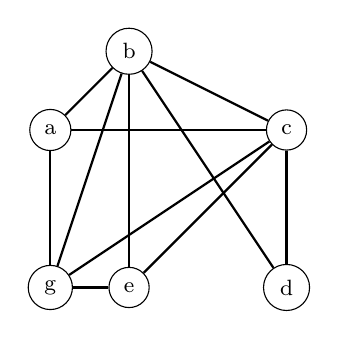
\begin{tikzpicture}
      \begin{scope}[every node/.style={draw=black,circle}]
        \node (a) at ( 0, 1) {\footnotesize e};
        \node (b) at ( 0, 4) {\footnotesize b};
        \node (c) at ( 2, 1) {\footnotesize d};
        \node (d) at ( 2, 3) {\footnotesize c};
        \node (e) at (-1, 1) {\footnotesize g};
        \node (f) at (-1, 3) {\footnotesize a};
      \end{scope}
      \begin{scope}[every edge/.style={draw=black,thick}]
        \path (a) edge (b);
        \path (a) edge (d);
        \path (a) edge (e);
        \path (b) edge (c);
        \path (b) edge (d);
        \path (b) edge (e);
        \path (b) edge (f);
        \path (c) edge (d);
        \path (d) edge (e);           
        \path (d) edge (f);
        \path (e) edge (f);
      \end{scope}
    \end{tikzpicture}
  \end{center}
  \begin{center}
    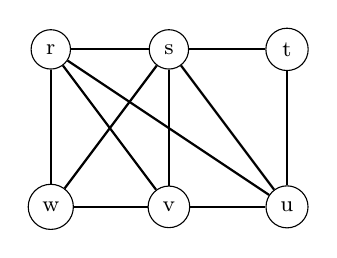
\begin{tikzpicture}
      \begin{scope}[every node/.style={draw=black,circle}]
        \node (a) at (0  ,0) {\footnotesize w};
        \node (b) at (0  ,2) {\footnotesize r};
        \node (c) at (1.5,0) {\footnotesize v};
        \node (d) at (1.5,2) {\footnotesize s};
        \node (e) at (3  ,0) {\footnotesize u};
        \node (f) at (3  ,2) {\footnotesize t};
      \end{scope}
      \begin{scope}[every edge/.style={draw=black,thick}]
        \path (a) edge (b);
        \path (a) edge (c);
        \path (c) edge (e);
        \path (a) edge (d);
        \path (b) edge (c);
        \path (b) edge (d);
        \path (b) edge (e);
        \path (b) edge (d);
        \path (d) edge (f);
        \path (c) edge (d);
        \path (d) edge (e);	            
        \path (e) edge (f);
      \end{scope}
    \end{tikzpicture}
  \end{center}
    
  \section*{No of maps}
    \(f(a) \rightarrow 6\) choices; \(f(b) \rightarrow 5\) choices; \(f(c) \rightarrow 4\) choices; etc.
    So, \(n!\) maps between the vertex sets of two graphs with \(n\) vertices.
  
  \section*{Some invariants}
    \begin{itemize}
      \item Degrees.
      \item Paths.
      \item Connection.
    \end{itemize}

  \section*{Adjacency matrix}
    Fix a listing of \(V\).
    \([a_{ij}]\) where \(a_{ij}\) is 1 if \(\{v_i,v_j\} \in E \) else 0.
  
  \section*{Example}
  \[
    \begin{bmatrix}
      0 & 1 & 1 & 0 & 0 & 1 \\
      1 & 0 & 1 & 1 & 1 & 1 \\
      1 & 1 & 0 & 1 & 1 & 1 \\
      0 & 1 & 1 & 0 & 0 & 0 \\
      0 & 1 & 1 & 0 & 0 & 1 \\
      1 & 1 & 1 & 0 & 1 & 0 
    \end{bmatrix}
    \qquad
    \begin{bmatrix}
      0 & 1 & 0 & 1 & 1 & 1 \\
      1 & 0 & 1 & 1 & 1 & 1 \\
      0 & 1 & 0 & 1 & 0 & 0 \\
      1 & 1 & 1 & 0 & 1 & 0 \\
      1 & 1 & 0 & 1 & 0 & 1 \\
      1 & 1 & 0 & 0 & 1 & 0 \\
    \end{bmatrix}
  \]

  \section*{Permutation matrix}
  Isomorphic \(\leftrightarrow\) \(\exists P\) such that \(A = PBP^\intercal\).

  \[
    \begin{bmatrix}
      0 & 1 & 0 & 0 \\
      1 & 0 & 0 & 0 \\
      0 & 0 & 1 & 0 \\
      0 & 0 & 0 & 1 \\
    \end{bmatrix}
    \begin{bmatrix}
      0 & 1 & 1 & 1 \\
      1 & 0 & 0 & 0 \\
      1 & 0 & 0 & 1 \\
      1 & 0 & 1 & 0 \\
    \end{bmatrix}
    \begin{bmatrix}
      0 & 1 & 0 & 0 \\
      1 & 0 & 0 & 0 \\
      0 & 0 & 1 & 0 \\
      0 & 0 & 0 & 1 \\
    \end{bmatrix} \]
    \[ =
    \begin{bmatrix}
      0 & 1 & 0 & 0 \\
      1 & 0 & 1 & 1 \\
      0 & 1 & 0 & 1 \\
      0 & 1 & 1 & 0 \\
    \end{bmatrix}        
  \]


  \section*{Binary encoding}
  \[
    \begin{bmatrix}
      0 & 1 & 1 & 0 & 0 & 1 \\
      {\color{atuorange} 1} & 0 & 1 & 1 & 1 & 1 \\
      {\color{atuorange} 1} & {\color{atuorange} 1} & 0 & 1 & 1 & 1 \\
      {\color{atuorange} 0} & {\color{atuorange} 1} & {\color{atuorange} 1} & 0 & 0 & 0 \\
      {\color{atuorange} 0} & {\color{atuorange} 1} & {\color{atuorange} 1} & {\color{atuorange} 0} & 0 & 1 \\
      {\color{atuorange} 1} & {\color{atuorange} 1} & {\color{atuorange} 1} & {\color{atuorange} 0} & {\color{atuorange} 1} & 0 
    \end{bmatrix}\]

    \[ \rightarrow 011001101111110111011000011001111010 \]
    \[ \textrm{or } { \color{atuorange} 111011011011101 } \]

  \section*{Decision problem}
    \[f(110101,101011) \rightarrow \textrm{Yes}\]
    \[f(111011011011101,1011111101110011) \rightarrow \textrm{No}\]
    \[f:\{0,1\}^* \times \{0,1\}^* \rightarrow \{0,1\} = 1 \textrm{ iff isomorphic} \]

    \[ \mathbf{GRAPHISO} = \{(G_1, G_2) | f(G_1, G_2) = 1\} \]

  %\printbibliography
\end{document} 